% Supernova Detection Poster - First Half (Procedure & ML Algorithm)
% Compile with: pdflatex poster_supernova.tex
\documentclass[25pt, a0paper, portrait]{tikzposter}

\usepackage{amsmath}
\usepackage{graphicx}
\usepackage{booktabs}
\usepackage{enumitem}
\usepackage{tikz}
\usetikzlibrary{arrows.meta, positioning, shapes.geometric, fit}

% Color theme
\definecolorpalette{AstroColors}{
    \definecolor{colorOne}{HTML}{1B2A4A}    % Dark navy
    \definecolor{colorTwo}{HTML}{2E5090}    % Medium blue
    \definecolor{colorThree}{HTML}{E8EEF7}  % Light blue
}

\defineblockstyle{AstroBlock}{
    titlewidthscale=1.0,
    bodywidthscale=1.0,
    titlecenter,
    titleoffsetx=0pt,
    titleoffsety=0pt,
    bodyoffsetx=0pt,
    bodyoffsety=0pt,
    bodyverticalshift=0pt,
    roundedcorners=10,
    linewidth=2pt,
    titleinnersep=8mm,
    bodyinnersep=8mm
}{
    \draw[color=colorTwo, fill=colorThree, rounded corners=\blockroundedcorners, line width=\blocklinewidth]
        (blockbody.south west) rectangle (blockbody.north east);
    \ifBlockHasTitle
        \draw[color=colorOne, fill=colorTwo, rounded corners=\blockroundedcorners, line width=\blocklinewidth]
        (blocktitle.south west) rectangle (blocktitle.north east);
    \fi
}

\usetheme{Default}
\usecolorstyle[colorPalette=AstroColors]{Britain}
\useblockstyle{AstroBlock}

% Title
\title{\parbox{\linewidth}{\centering
    Automated Detection of Supernovae in the COSMOS Field\\
    by Comparing JWST and HST Images with Deep Learning}}
\author{N. Suzuki}
\institute{} % Add your institution
\date{}

\begin{document}
\maketitle

% ============================================================
% Row 1: Introduction + Data
% ============================================================

\begin{columns}
\column{0.48}

\block{1. Introduction}{
    Supernovae (SNe) are rare transient events --- bright stellar explosions
    that appear as new point sources near their host galaxies. Detecting them
    requires comparing observations of the same field taken at different epochs.

    \vspace{4mm}
    \textbf{Challenge:}
    \begin{itemize}[leftmargin=*, itemsep=2mm]
        \item The COSMOS field was observed by both HST (2004--2005)
              and JWST (2023--2024), spanning $\sim$20 years
        \item Images come from different telescopes with different
              pixel scales, filters, and resolutions
        \item Manual inspection of $\sim$212,000 objects is infeasible
        \item SN rate is very low: $\sim$1 per 1,000 objects
    \end{itemize}

    \vspace{4mm}
    \textbf{Goal:} Build an automated CNN-based pipeline to detect
    SN candidates by comparing HST and JWST image triplets, validated
    against 23 visually confirmed supernovae.
}

\column{0.48}

\block{2. Data}{
    \textbf{HST COSMOS-ACS:} 212,460 PNG cutouts\\
    \hspace*{5mm} Filename: \texttt{\{ID\}\_\{Field\}\_hstcosmos.png}\\[2mm]
    \textbf{JWST COSMOS-Web:} 424,941 PNG cutouts (2 filters per object)\\
    \hspace*{5mm} Filenames: \texttt{\{ID\}\_\{Field\}\_jwst1.png},
                             \texttt{\{ID\}\_\{Field\}\_jwst2.png}\\[2mm]
    \textbf{Matching:} By object ID (field names may differ between HST/JWST)\\[2mm]
    \textbf{Image properties:}
    \begin{itemize}[leftmargin=*, itemsep=2mm]
        \item Galaxy centered in each PNG cutout
        \item Grayscale, various sizes --- resized to $64 \times 64$ pixels
        \item Central 50\% cropped to focus on galaxy region
    \end{itemize}

    \vspace{4mm}
    \textbf{Training set:}
    23 visually confirmed supernovae used for validation and training.

    \vspace{4mm}
    \begin{center}
    \begin{tabular}{lrl}
        \toprule
        \textbf{Dataset} & \textbf{Count} & \textbf{Telescope} \\
        \midrule
        HST images          & 212,460 & HST ACS/WFC \\
        JWST images         & 424,941 & JWST NIRCam \\
        Matched triplets    & $\sim$212,000 & HST + JWST1 + JWST2 \\
        Known supernovae    & 23 & Visual inspection \\
        Expected SN rate    & $\sim$1/1000 & \\
        \bottomrule
    \end{tabular}
    \end{center}
}

\end{columns}

% ============================================================
% Row 2: Physical Constraints + Method
% ============================================================

\begin{columns}
\column{0.48}

\block{3. Physical Constraints}{
    Key physical priors are built into the detection algorithm:

    \vspace{4mm}
    \textbf{(a) SN appears near host galaxy}\\[2mm]
    A supernova is an exploding star within a galaxy. It must appear
    near the center of each PNG cutout (where the host galaxy is).
    We crop the central 50\% of each image and only consider sources
    within 25\% of image center.

    \vspace{6mm}
    \textbf{(b) SN must be consistent across filters}

    \vspace{4mm}
    \begin{center}
    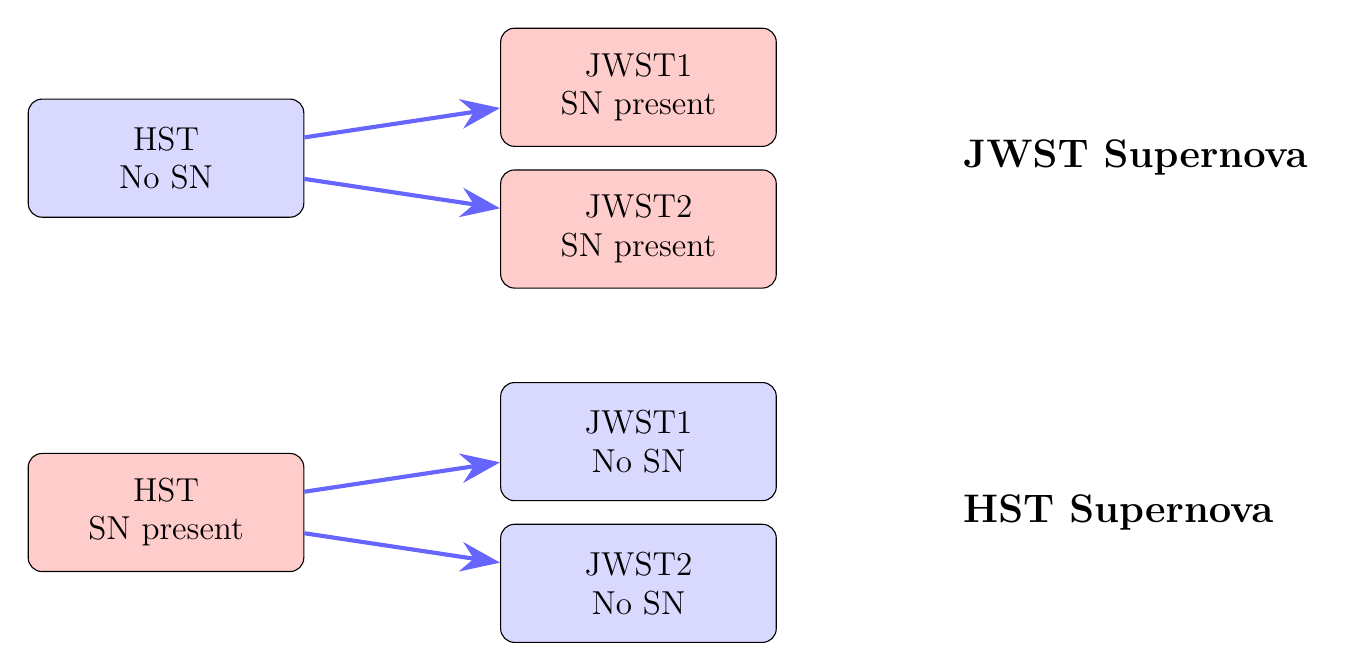
\begin{tikzpicture}[
        box/.style={draw, rounded corners=5pt, minimum width=3.5cm,
                    minimum height=1.5cm, align=center, font=\large},
        arr/.style={-{Stealth[length=5mm]}, line width=1.5pt}
    ]
        % JWST SN
        \node[box, fill=blue!15] (hst1) at (0, 0) {HST\\No SN};
        \node[box, fill=red!20] (jwst1a) at (6, 0.9) {JWST1\\SN present};
        \node[box, fill=red!20] (jwst1b) at (6, -0.9) {JWST2\\SN present};
        \node[font=\Large\bfseries, right] at (10, 0) {JWST Supernova};

        % HST SN
        \node[box, fill=red!20] (hst2) at (0, -4.5) {HST\\SN present};
        \node[box, fill=blue!15] (jwst2a) at (6, -3.6) {JWST1\\No SN};
        \node[box, fill=blue!15] (jwst2b) at (6, -5.4) {JWST2\\No SN};
        \node[font=\Large\bfseries, right] at (10, -4.5) {HST Supernova};

        \draw[arr, blue!60] (hst1) -- (jwst1a);
        \draw[arr, blue!60] (hst1) -- (jwst1b);
        \draw[arr, blue!60] (hst2) -- (jwst2a);
        \draw[arr, blue!60] (hst2) -- (jwst2b);
    \end{tikzpicture}
    \end{center}

    \vspace{4mm}
    \begin{itemize}[leftmargin=*, itemsep=2mm]
        \item \textbf{JWST SN:} new source in \textit{both} JWST1 and JWST2
              (at the same position), but absent in HST
        \item \textbf{HST SN:} source in HST only, absent in
              \textit{both} JWST1 and JWST2 (SN faded by JWST epoch)
        \item Requiring detection in both JWST filters eliminates
              single-filter artifacts and noise
    \end{itemize}
}

\column{0.48}

\block{4. CNN Architecture \& Training}{
    \textbf{Input:} 3-channel $64 \times 64$ image (HST + JWST1 + JWST2)\\
    \textbf{Output:} Probability of supernova (0 to 1)

    \vspace{4mm}
    \begin{center}
    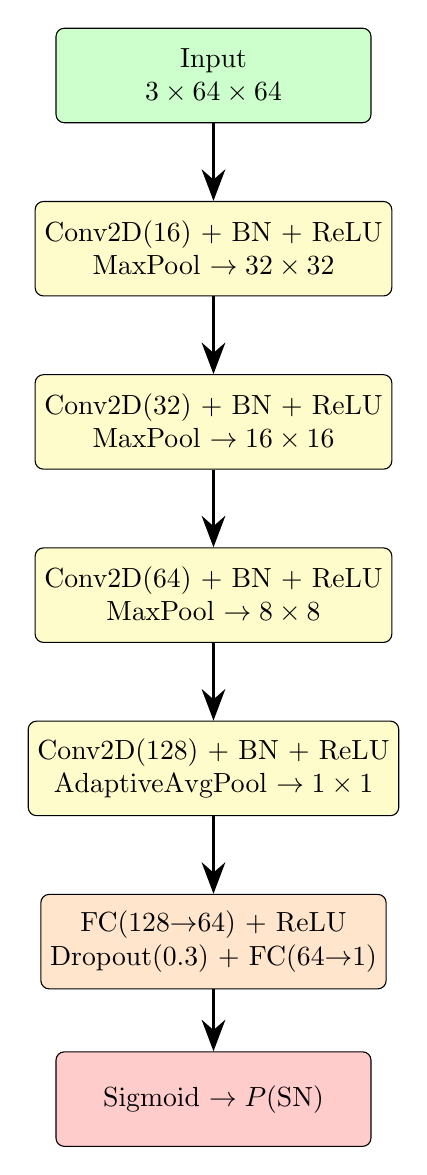
\begin{tikzpicture}[
        layer/.style={draw, rounded corners=3pt, minimum height=1.2cm,
                      align=center, font=\normalsize},
        arr/.style={-{Stealth[length=4mm]}, line width=1.2pt}
    ]
        \node[layer, fill=green!20, minimum width=4cm] (input) at (0, 0)
            {Input\\$3 \times 64 \times 64$};
        \node[layer, fill=yellow!20, minimum width=4cm] (conv1) at (0, -2.2)
            {Conv2D(16) + BN + ReLU\\MaxPool $\rightarrow 32 \times 32$};
        \node[layer, fill=yellow!20, minimum width=4cm] (conv2) at (0, -4.4)
            {Conv2D(32) + BN + ReLU\\MaxPool $\rightarrow 16 \times 16$};
        \node[layer, fill=yellow!20, minimum width=4cm] (conv3) at (0, -6.6)
            {Conv2D(64) + BN + ReLU\\MaxPool $\rightarrow 8 \times 8$};
        \node[layer, fill=yellow!20, minimum width=4cm] (conv4) at (0, -8.8)
            {Conv2D(128) + BN + ReLU\\AdaptiveAvgPool $\rightarrow 1 \times 1$};
        \node[layer, fill=orange!20, minimum width=4cm] (fc) at (0, -11.0)
            {FC(128$\rightarrow$64) + ReLU\\Dropout(0.3) + FC(64$\rightarrow$1)};
        \node[layer, fill=red!20, minimum width=4cm] (out) at (0, -13.0)
            {Sigmoid $\rightarrow P(\text{SN})$};

        \foreach \a/\b in {input/conv1, conv1/conv2, conv2/conv3, conv3/conv4, conv4/fc, fc/out}
            \draw[arr] (\a) -- (\b);
    \end{tikzpicture}
    \end{center}

    \vspace{4mm}
    \textbf{Training strategy:}
    \begin{itemize}[leftmargin=*, itemsep=2mm]
        \item 23 known SN oversampled $\times 50$ as real positives
        \item 5,000 artificial SN injected as Gaussian point sources
              near the galaxy center (both JWST-type and HST-type)
        \item 100,000 negatives (20:1 ratio) from non-SN objects
        \item Loss: Binary Cross-Entropy with Logits
        \item Optimizer: Adam, LR = $10^{-3}$, ReduceLROnPlateau
        \item Augmentation: random flips + 90$^\circ$ rotations
        \item 50 epochs, best model saved by known SN recovery rate
    \end{itemize}
}

\end{columns}

% ============================================================
% Row 3: Pipeline + Threshold Selection
% ============================================================

\begin{columns}
\column{0.48}

\block{5. Detection Pipeline}{
    \begin{center}
    \begin{tikzpicture}[
        step/.style={draw, rounded corners=5pt, minimum width=12cm,
                     minimum height=1.8cm, align=center, font=\Large},
        arr/.style={-{Stealth[length=5mm]}, line width=2pt, colorTwo}
    ]
        \node[step, fill=green!15] (s1) at (0, 0)
            {\textbf{Step 1:} Match HST + JWST1 + JWST2 by object ID};
        \node[step, fill=yellow!15] (s2) at (0, -3)
            {\textbf{Step 2:} Train CNN on known SN + artificial SN};
        \node[step, fill=orange!15] (s3) at (0, -6)
            {\textbf{Step 3:} Validate --- recover ALL 23 known SN};
        \node[step, fill=red!15] (s4) at (0, -9)
            {\textbf{Step 4:} Apply to all $\sim$212,000 objects};
        \node[step, fill=blue!15] (s5) at (0, -12)
            {\textbf{Step 5:} Verify known SN in results; check rate $\sim$1/1000};

        \foreach \a/\b in {s1/s2, s2/s3, s3/s4, s4/s5}
            \draw[arr] (\a) -- (\b);
    \end{tikzpicture}
    \end{center}

    \vspace{4mm}
    Candidates are written to disk \textit{immediately} as they are found,
    allowing real-time monitoring during the multi-hour inference run.
}

\column{0.48}

\block{6. Threshold Selection \& Artificial SN}{
    \textbf{Automatic threshold:}\\
    The classification threshold is set to 90\% of the lowest probability
    among the 23 known supernovae. This guarantees 100\% recovery of
    all confirmed SN while minimizing false positives.

    \vspace{4mm}
    $$\theta = 0.9 \times \min_{i \in \text{known}} P_i(\text{SN})$$

    \vspace{4mm}
    \textbf{Artificial supernova injection:}\\
    Gaussian point sources are injected near the galaxy center to
    augment the small training set:

    $$I_{\text{SN}}(x, y) = I_{\text{orig}}(x, y) + A \cdot
    \exp\!\left(-\frac{(x - x_0)^2 + (y - y_0)^2}{2\sigma^2}\right)$$

    where:
    \begin{itemize}[leftmargin=*, itemsep=2mm]
        \item $(x_0, y_0)$: random position within 25\% of image center
        \item $A \in [0.3, 0.9]$: peak brightness (random)
        \item $\sigma \in [1.0, 3.0]$ pixels: PSF width (random)
        \item For JWST SN: injected at \textit{same position} in both
              filters with slightly different brightness
              ($A_2 = A_1 \times U[0.7, 1.3]$)
    \end{itemize}

    \vspace{4mm}
    \textit{[Space reserved for artificial SN example images]}
}

\end{columns}

% ============================================================
% Bottom: Results placeholder
% ============================================================

\block{7. Results}{
    \vspace{2mm}
    \textit{[Second half of poster --- to be filled with result images,
    candidate gallery, detection statistics, and recovery plots.]}
    \vspace{2mm}
}

\end{document}
